\reportsection{Provenance: From Retrofit to Parametrisation Model}
\label{sec:provenance}

The first phase of this work compared the existing
\textsf{Arkworks/crypto-primitives} Merkle tree with the Chiesa--Yogev
presentation~\cite{CY26}.  It began as implementation work around open feature
requests: simplify the split hash interface, remove caller-side ordering
footguns, support richer tree shapes, and compress multi-openings.  Read
together, those requests pointed to one broader issue.  The implementation had
many locally reasonable decisions, but no single specification against which
their combined behaviour could be reviewed.

That comparison produced concrete engineering results.  The \code{CoSet}
multiproof encoding realises the book's path-pruning optimisation for
multi-openings, and \code{ImplicitCoPath} performs the same pruning without
materialising a coordinate bookkeeping layer, which is purely pedagogical when
used outside a position-tagging context.  That coordinate-encoding backing was nonetheless built out
in full, and although it sits outside this report's use, it is exactly the
groundwork the geometric, position-tagged style of binding
(\cref{sec:binding}) would build on.  The
\code{Committed}/\code{OpeningProof}/\code{Opening} split makes ordering and
duplicate-index validation part of construction rather than caller discipline.
\Cref{fig:coset-compression} shows the headline measurement: at $4{,}096$
opened leaves the clustered multiproof is roughly a tenth the size of the
per-path encoding it replaces.  The benchmark harnesses built to take that
measurement prefigure the cost benchmarks of \cref{sec:cost}.  None of this code
was merged into the current tree.

\begin{figure}[t]
  \centering
  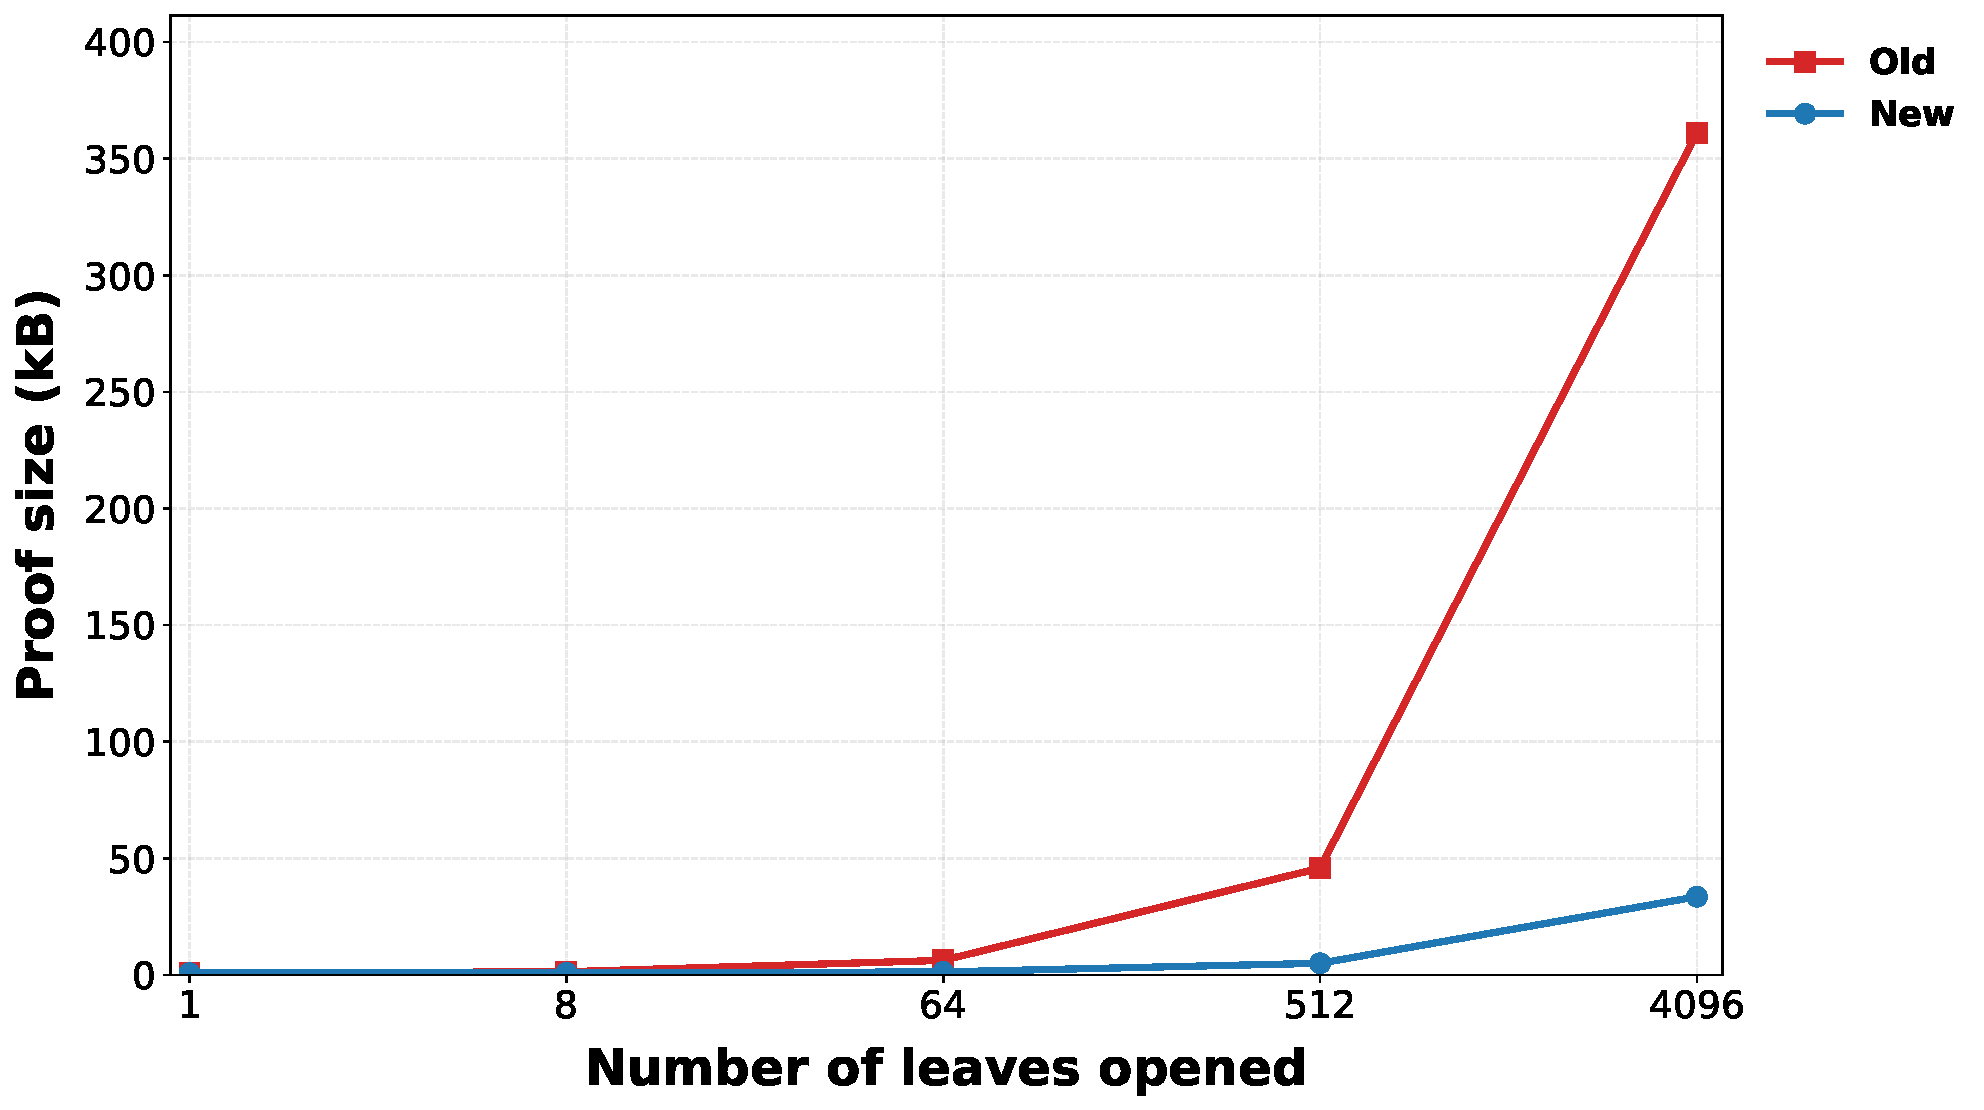
\includegraphics[width=0.5\linewidth]{figures/coset-proof-size-clustered.pdf}
  \caption{Phase-1 multiproof compression on clustered openings of a
  $4{,}096$-leaf tree.  The \code{CoSet} encoding prunes shared path material,
  so proof size grows with the disclosed frontier rather than with the number
  of individual paths: at $4{,}096$ opened leaves the compressed proof is
  roughly $33$\,kB against roughly $360$\,kB uncompressed.}
  \label{fig:coset-compression}
\end{figure}

The stronger finding was methodological.  A reference definition can organise
an API, yet an API alone still does not tell a developer which security claim a
concrete configuration supports.  That is the step from retrofit to
parametrisation model: keep the literature-facing definition, connect it to
executable interfaces, state the security games, derive the parameters, and
expose the evidence boundary.  What the semester enabled therefore runs through
the whole report.  The freedoms whose absence the retrofit exposed (simpler
hash interfaces, variable tree shapes, efficient multi-opening compression) are
exactly the ones the parametrisation model of \cref{sec:spine} grants and then
guards.  The multiproof pruning strategy survives in \textsf{ark-mt}'s capped
openings, where the commitment publishes the ordered digest layer at a chosen
depth instead of the single root, so every opening sheds that many layers of
shared copath.  The cost measurements of \cref{sec:cost} run on the
benchmarking craft built here.
